\documentclass[tikz]{standalone}
\usepackage{tikz}
\usetikzlibrary{positioning}

\begin{document}
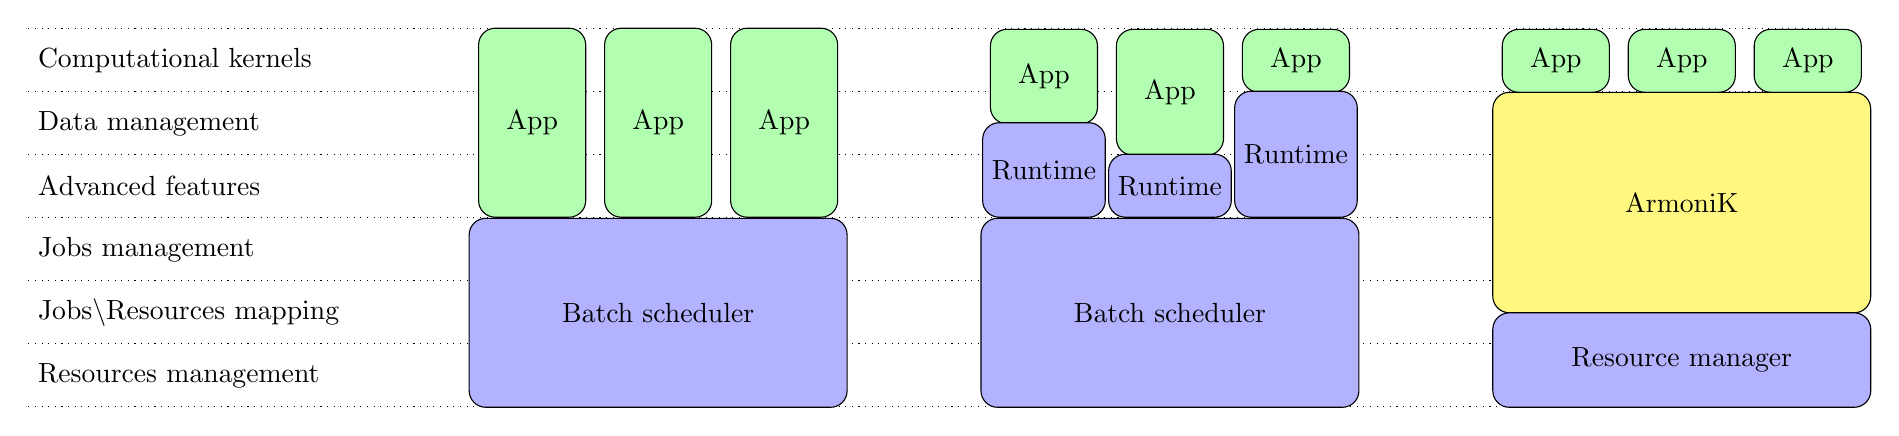
\begin{tikzpicture}[rounded corners=2pt]

% Sizes
\def\appw{1.6}
\def\apph{0.8}
\def\gap{0.85}

% Add some dotted lines as guide
\foreach \y in {4, 3.2, 2.4, 1.6, 0.8, 0, -0.8} {
    \draw[dotted] (-8,\y) -- (15,\y);
}

% Scheduler properties
\foreach \i/\text in {
3.6/Computational kernels,
2.8/Data management,
2/Advanced features,
1.2/Jobs management,
0.4/Jobs\textbackslash Resources mapping,
-0.4/Resources management
} {
  \node[anchor=west] at (-8,\i) {\text};
}

% Batch only
\foreach \i in {-1,0,1} {
  \node[draw, fill=green!30, minimum width=\appw*\gap cm, minimum height=3 * \apph cm, anchor=south, rounded corners=6pt]
        at (\i*\appw,1.6) {App};
}
\node[draw, fill=blue!30, minimum width=3 * \appw cm, minimum height=3 * \apph cm, anchor=north, rounded corners=6pt]
      at (0,1.6) {Batch scheduler};

% Batch + Runtime
\node[draw, fill=green!30, minimum width=\appw*\gap cm, minimum height=1.2cm, anchor=north, rounded corners=6pt]
        at (-1 * \appw + 6.5,4) {App};
\node[draw, fill=blue!30, minimum width=\appw*\gap cm, minimum height=1.2cm,, anchor=south, rounded corners=6pt]
        at (-1 * \appw + 6.5,1.6) {Runtime};

\node[draw, fill=green!30, minimum width=\appw*\gap cm, minimum height=2*\apph cm, anchor=north, rounded corners=6pt]
        at (0 * \appw + 6.5,4) {App};
\node[draw, fill=blue!30, minimum width=\appw*\gap cm, minimum height=\apph cm,, anchor=south, rounded corners=6pt]
        at (0 * \appw + 6.5,1.6) {Runtime};

\node[draw, fill=green!30, minimum width=\appw*\gap cm, minimum height=\apph cm, anchor=north, rounded corners=6pt]
        at (1 * \appw + 6.5,4) {App};
\node[draw, fill=blue!30, minimum width=\appw*\gap cm, minimum height=2*\apph cm,, anchor=south, rounded corners=6pt]
        at (1 * \appw + 6.5,1.6) {Runtime};

\node[draw, fill=blue!30, minimum width=3 * \appw cm, minimum height=3 * \apph cm, anchor=north, rounded corners=6pt]
      at (6.5,1.6) {Batch scheduler};

% ArmoniK + Resource Manager
\foreach \i in {-1,0,1} {
  \node[draw, fill=green!30, minimum width=\appw*\gap cm, minimum height=\apph cm, anchor=north,rounded corners=6pt]
        at (\i*\appw + 13,4) {App};
}
\node[draw, fill=yellow!50, minimum width=3 * \appw cm, minimum height=2.8cm, anchor=north, rounded corners=6pt]
      at (13,3.2) {ArmoniK};
\node[draw, fill=blue!30, minimum width=3 * \appw cm, minimum height=1.2cm, anchor=north, rounded corners=6pt]
      at (13,0.4) {Resource manager};

\end{tikzpicture}
\end{document}
